\documentclass{article} % For LaTeX2e
\usepackage{iclr2027_conference,times}

%%%%% NEW MATH DEFINITIONS %%%%%

\usepackage{amsmath,amsfonts,bm}

% Mark sections of captions for referring to divisions of figures
\newcommand{\figleft}{{\em (Left)}}
\newcommand{\figcenter}{{\em (Center)}}
\newcommand{\figright}{{\em (Right)}}
\newcommand{\figtop}{{\em (Top)}}
\newcommand{\figbottom}{{\em (Bottom)}}
\newcommand{\captiona}{{\em (a)}}
\newcommand{\captionb}{{\em (b)}}
\newcommand{\captionc}{{\em (c)}}
\newcommand{\captiond}{{\em (d)}}

% Highlight a newly defined term
\newcommand{\newterm}[1]{{\bf #1}}


% Figure reference, lower-case.
\def\figref#1{figure~\ref{#1}}
% Figure reference, capital. For start of sentence
\def\Figref#1{Figure~\ref{#1}}
\def\twofigref#1#2{figures \ref{#1} and \ref{#2}}
\def\quadfigref#1#2#3#4{figures \ref{#1}, \ref{#2}, \ref{#3} and \ref{#4}}
% Section reference, lower-case.
\def\secref#1{section~\ref{#1}}
% Section reference, capital.
\def\Secref#1{Section~\ref{#1}}
% Reference to two sections.
\def\twosecrefs#1#2{sections \ref{#1} and \ref{#2}}
% Reference to three sections.
\def\secrefs#1#2#3{sections \ref{#1}, \ref{#2} and \ref{#3}}
% Reference to an equation, lower-case.
\def\eqref#1{equation~\ref{#1}}
% Reference to an equation, upper case
\def\Eqref#1{Equation~\ref{#1}}
% A raw reference to an equation---avoid using if possible
\def\plaineqref#1{\ref{#1}}
% Reference to a chapter, lower-case.
\def\chapref#1{chapter~\ref{#1}}
% Reference to an equation, upper case.
\def\Chapref#1{Chapter~\ref{#1}}
% Reference to a range of chapters
\def\rangechapref#1#2{chapters\ref{#1}--\ref{#2}}
% Reference to an algorithm, lower-case.
\def\algref#1{algorithm~\ref{#1}}
% Reference to an algorithm, upper case.
\def\Algref#1{Algorithm~\ref{#1}}
\def\twoalgref#1#2{algorithms \ref{#1} and \ref{#2}}
\def\Twoalgref#1#2{Algorithms \ref{#1} and \ref{#2}}
% Reference to a part, lower case
\def\partref#1{part~\ref{#1}}
% Reference to a part, upper case
\def\Partref#1{Part~\ref{#1}}
\def\twopartref#1#2{parts \ref{#1} and \ref{#2}}

\def\ceil#1{\lceil #1 \rceil}
\def\floor#1{\lfloor #1 \rfloor}
\def\1{\bm{1}}
\newcommand{\train}{\mathcal{D}}
\newcommand{\valid}{\mathcal{D_{\mathrm{valid}}}}
\newcommand{\test}{\mathcal{D_{\mathrm{test}}}}

\def\eps{{\epsilon}}


% Random variables
\def\reta{{\textnormal{$\eta$}}}
\def\ra{{\textnormal{a}}}
\def\rb{{\textnormal{b}}}
\def\rc{{\textnormal{c}}}
\def\rd{{\textnormal{d}}}
\def\re{{\textnormal{e}}}
\def\rf{{\textnormal{f}}}
\def\rg{{\textnormal{g}}}
\def\rh{{\textnormal{h}}}
\def\ri{{\textnormal{i}}}
\def\rj{{\textnormal{j}}}
\def\rk{{\textnormal{k}}}
\def\rl{{\textnormal{l}}}
% rm is already a command, just don't name any random variables m
\def\rn{{\textnormal{n}}}
\def\ro{{\textnormal{o}}}
\def\rp{{\textnormal{p}}}
\def\rq{{\textnormal{q}}}
\def\rr{{\textnormal{r}}}
\def\rs{{\textnormal{s}}}
\def\rt{{\textnormal{t}}}
\def\ru{{\textnormal{u}}}
\def\rv{{\textnormal{v}}}
\def\rw{{\textnormal{w}}}
\def\rx{{\textnormal{x}}}
\def\ry{{\textnormal{y}}}
\def\rz{{\textnormal{z}}}

% Random vectors
\def\rvepsilon{{\mathbf{\epsilon}}}
\def\rvtheta{{\mathbf{\theta}}}
\def\rva{{\mathbf{a}}}
\def\rvb{{\mathbf{b}}}
\def\rvc{{\mathbf{c}}}
\def\rvd{{\mathbf{d}}}
\def\rve{{\mathbf{e}}}
\def\rvf{{\mathbf{f}}}
\def\rvg{{\mathbf{g}}}
\def\rvh{{\mathbf{h}}}
\def\rvu{{\mathbf{i}}}
\def\rvj{{\mathbf{j}}}
\def\rvk{{\mathbf{k}}}
\def\rvl{{\mathbf{l}}}
\def\rvm{{\mathbf{m}}}
\def\rvn{{\mathbf{n}}}
\def\rvo{{\mathbf{o}}}
\def\rvp{{\mathbf{p}}}
\def\rvq{{\mathbf{q}}}
\def\rvr{{\mathbf{r}}}
\def\rvs{{\mathbf{s}}}
\def\rvt{{\mathbf{t}}}
\def\rvu{{\mathbf{u}}}
\def\rvv{{\mathbf{v}}}
\def\rvw{{\mathbf{w}}}
\def\rvx{{\mathbf{x}}}
\def\rvy{{\mathbf{y}}}
\def\rvz{{\mathbf{z}}}

% Elements of random vectors
\def\erva{{\textnormal{a}}}
\def\ervb{{\textnormal{b}}}
\def\ervc{{\textnormal{c}}}
\def\ervd{{\textnormal{d}}}
\def\erve{{\textnormal{e}}}
\def\ervf{{\textnormal{f}}}
\def\ervg{{\textnormal{g}}}
\def\ervh{{\textnormal{h}}}
\def\ervi{{\textnormal{i}}}
\def\ervj{{\textnormal{j}}}
\def\ervk{{\textnormal{k}}}
\def\ervl{{\textnormal{l}}}
\def\ervm{{\textnormal{m}}}
\def\ervn{{\textnormal{n}}}
\def\ervo{{\textnormal{o}}}
\def\ervp{{\textnormal{p}}}
\def\ervq{{\textnormal{q}}}
\def\ervr{{\textnormal{r}}}
\def\ervs{{\textnormal{s}}}
\def\ervt{{\textnormal{t}}}
\def\ervu{{\textnormal{u}}}
\def\ervv{{\textnormal{v}}}
\def\ervw{{\textnormal{w}}}
\def\ervx{{\textnormal{x}}}
\def\ervy{{\textnormal{y}}}
\def\ervz{{\textnormal{z}}}

% Random matrices
\def\rmA{{\mathbf{A}}}
\def\rmB{{\mathbf{B}}}
\def\rmC{{\mathbf{C}}}
\def\rmD{{\mathbf{D}}}
\def\rmE{{\mathbf{E}}}
\def\rmF{{\mathbf{F}}}
\def\rmG{{\mathbf{G}}}
\def\rmH{{\mathbf{H}}}
\def\rmI{{\mathbf{I}}}
\def\rmJ{{\mathbf{J}}}
\def\rmK{{\mathbf{K}}}
\def\rmL{{\mathbf{L}}}
\def\rmM{{\mathbf{M}}}
\def\rmN{{\mathbf{N}}}
\def\rmO{{\mathbf{O}}}
\def\rmP{{\mathbf{P}}}
\def\rmQ{{\mathbf{Q}}}
\def\rmR{{\mathbf{R}}}
\def\rmS{{\mathbf{S}}}
\def\rmT{{\mathbf{T}}}
\def\rmU{{\mathbf{U}}}
\def\rmV{{\mathbf{V}}}
\def\rmW{{\mathbf{W}}}
\def\rmX{{\mathbf{X}}}
\def\rmY{{\mathbf{Y}}}
\def\rmZ{{\mathbf{Z}}}

% Elements of random matrices
\def\ermA{{\textnormal{A}}}
\def\ermB{{\textnormal{B}}}
\def\ermC{{\textnormal{C}}}
\def\ermD{{\textnormal{D}}}
\def\ermE{{\textnormal{E}}}
\def\ermF{{\textnormal{F}}}
\def\ermG{{\textnormal{G}}}
\def\ermH{{\textnormal{H}}}
\def\ermI{{\textnormal{I}}}
\def\ermJ{{\textnormal{J}}}
\def\ermK{{\textnormal{K}}}
\def\ermL{{\textnormal{L}}}
\def\ermM{{\textnormal{M}}}
\def\ermN{{\textnormal{N}}}
\def\ermO{{\textnormal{O}}}
\def\ermP{{\textnormal{P}}}
\def\ermQ{{\textnormal{Q}}}
\def\ermR{{\textnormal{R}}}
\def\ermS{{\textnormal{S}}}
\def\ermT{{\textnormal{T}}}
\def\ermU{{\textnormal{U}}}
\def\ermV{{\textnormal{V}}}
\def\ermW{{\textnormal{W}}}
\def\ermX{{\textnormal{X}}}
\def\ermY{{\textnormal{Y}}}
\def\ermZ{{\textnormal{Z}}}

% Vectors
\def\vzero{{\bm{0}}}
\def\vone{{\bm{1}}}
\def\vmu{{\bm{\mu}}}
\def\vtheta{{\bm{\theta}}}
\def\va{{\bm{a}}}
\def\vb{{\bm{b}}}
\def\vc{{\bm{c}}}
\def\vd{{\bm{d}}}
\def\ve{{\bm{e}}}
\def\vf{{\bm{f}}}
\def\vg{{\bm{g}}}
\def\vh{{\bm{h}}}
\def\vi{{\bm{i}}}
\def\vj{{\bm{j}}}
\def\vk{{\bm{k}}}
\def\vl{{\bm{l}}}
\def\vm{{\bm{m}}}
\def\vn{{\bm{n}}}
\def\vo{{\bm{o}}}
\def\vp{{\bm{p}}}
\def\vq{{\bm{q}}}
\def\vr{{\bm{r}}}
\def\vs{{\bm{s}}}
\def\vt{{\bm{t}}}
\def\vu{{\bm{u}}}
\def\vv{{\bm{v}}}
\def\vw{{\bm{w}}}
\def\vx{{\bm{x}}}
\def\vy{{\bm{y}}}
\def\vz{{\bm{z}}}

% Elements of vectors
\def\evalpha{{\alpha}}
\def\evbeta{{\beta}}
\def\evepsilon{{\epsilon}}
\def\evlambda{{\lambda}}
\def\evomega{{\omega}}
\def\evmu{{\mu}}
\def\evpsi{{\psi}}
\def\evsigma{{\sigma}}
\def\evtheta{{\theta}}
\def\eva{{a}}
\def\evb{{b}}
\def\evc{{c}}
\def\evd{{d}}
\def\eve{{e}}
\def\evf{{f}}
\def\evg{{g}}
\def\evh{{h}}
\def\evi{{i}}
\def\evj{{j}}
\def\evk{{k}}
\def\evl{{l}}
\def\evm{{m}}
\def\evn{{n}}
\def\evo{{o}}
\def\evp{{p}}
\def\evq{{q}}
\def\evr{{r}}
\def\evs{{s}}
\def\evt{{t}}
\def\evu{{u}}
\def\evv{{v}}
\def\evw{{w}}
\def\evx{{x}}
\def\evy{{y}}
\def\evz{{z}}

% Matrix
\def\mA{{\bm{A}}}
\def\mB{{\bm{B}}}
\def\mC{{\bm{C}}}
\def\mD{{\bm{D}}}
\def\mE{{\bm{E}}}
\def\mF{{\bm{F}}}
\def\mG{{\bm{G}}}
\def\mH{{\bm{H}}}
\def\mI{{\bm{I}}}
\def\mJ{{\bm{J}}}
\def\mK{{\bm{K}}}
\def\mL{{\bm{L}}}
\def\mM{{\bm{M}}}
\def\mN{{\bm{N}}}
\def\mO{{\bm{O}}}
\def\mP{{\bm{P}}}
\def\mQ{{\bm{Q}}}
\def\mR{{\bm{R}}}
\def\mS{{\bm{S}}}
\def\mT{{\bm{T}}}
\def\mU{{\bm{U}}}
\def\mV{{\bm{V}}}
\def\mW{{\bm{W}}}
\def\mX{{\bm{X}}}
\def\mY{{\bm{Y}}}
\def\mZ{{\bm{Z}}}
\def\mBeta{{\bm{\beta}}}
\def\mPhi{{\bm{\Phi}}}
\def\mLambda{{\bm{\Lambda}}}
\def\mSigma{{\bm{\Sigma}}}

% Tensor
\DeclareMathAlphabet{\mathsfit}{\encodingdefault}{\sfdefault}{m}{sl}
\SetMathAlphabet{\mathsfit}{bold}{\encodingdefault}{\sfdefault}{bx}{n}
\newcommand{\tens}[1]{\bm{\mathsfit{#1}}}
\def\tA{{\tens{A}}}
\def\tB{{\tens{B}}}
\def\tC{{\tens{C}}}
\def\tD{{\tens{D}}}
\def\tE{{\tens{E}}}
\def\tF{{\tens{F}}}
\def\tG{{\tens{G}}}
\def\tH{{\tens{H}}}
\def\tI{{\tens{I}}}
\def\tJ{{\tens{J}}}
\def\tK{{\tens{K}}}
\def\tL{{\tens{L}}}
\def\tM{{\tens{M}}}
\def\tN{{\tens{N}}}
\def\tO{{\tens{O}}}
\def\tP{{\tens{P}}}
\def\tQ{{\tens{Q}}}
\def\tR{{\tens{R}}}
\def\tS{{\tens{S}}}
\def\tT{{\tens{T}}}
\def\tU{{\tens{U}}}
\def\tV{{\tens{V}}}
\def\tW{{\tens{W}}}
\def\tX{{\tens{X}}}
\def\tY{{\tens{Y}}}
\def\tZ{{\tens{Z}}}


% Graph
\def\gA{{\mathcal{A}}}
\def\gB{{\mathcal{B}}}
\def\gC{{\mathcal{C}}}
\def\gD{{\mathcal{D}}}
\def\gE{{\mathcal{E}}}
\def\gF{{\mathcal{F}}}
\def\gG{{\mathcal{G}}}
\def\gH{{\mathcal{H}}}
\def\gI{{\mathcal{I}}}
\def\gJ{{\mathcal{J}}}
\def\gK{{\mathcal{K}}}
\def\gL{{\mathcal{L}}}
\def\gM{{\mathcal{M}}}
\def\gN{{\mathcal{N}}}
\def\gO{{\mathcal{O}}}
\def\gP{{\mathcal{P}}}
\def\gQ{{\mathcal{Q}}}
\def\gR{{\mathcal{R}}}
\def\gS{{\mathcal{S}}}
\def\gT{{\mathcal{T}}}
\def\gU{{\mathcal{U}}}
\def\gV{{\mathcal{V}}}
\def\gW{{\mathcal{W}}}
\def\gX{{\mathcal{X}}}
\def\gY{{\mathcal{Y}}}
\def\gZ{{\mathcal{Z}}}

% Sets
\def\sA{{\mathbb{A}}}
\def\sB{{\mathbb{B}}}
\def\sC{{\mathbb{C}}}
\def\sD{{\mathbb{D}}}
% Don't use a set called E, because this would be the same as our symbol
% for expectation.
\def\sF{{\mathbb{F}}}
\def\sG{{\mathbb{G}}}
\def\sH{{\mathbb{H}}}
\def\sI{{\mathbb{I}}}
\def\sJ{{\mathbb{J}}}
\def\sK{{\mathbb{K}}}
\def\sL{{\mathbb{L}}}
\def\sM{{\mathbb{M}}}
\def\sN{{\mathbb{N}}}
\def\sO{{\mathbb{O}}}
\def\sP{{\mathbb{P}}}
\def\sQ{{\mathbb{Q}}}
\def\sR{{\mathbb{R}}}
\def\sS{{\mathbb{S}}}
\def\sT{{\mathbb{T}}}
\def\sU{{\mathbb{U}}}
\def\sV{{\mathbb{V}}}
\def\sW{{\mathbb{W}}}
\def\sX{{\mathbb{X}}}
\def\sY{{\mathbb{Y}}}
\def\sZ{{\mathbb{Z}}}

% Entries of a matrix
\def\emLambda{{\Lambda}}
\def\emA{{A}}
\def\emB{{B}}
\def\emC{{C}}
\def\emD{{D}}
\def\emE{{E}}
\def\emF{{F}}
\def\emG{{G}}
\def\emH{{H}}
\def\emI{{I}}
\def\emJ{{J}}
\def\emK{{K}}
\def\emL{{L}}
\def\emM{{M}}
\def\emN{{N}}
\def\emO{{O}}
\def\emP{{P}}
\def\emQ{{Q}}
\def\emR{{R}}
\def\emS{{S}}
\def\emT{{T}}
\def\emU{{U}}
\def\emV{{V}}
\def\emW{{W}}
\def\emX{{X}}
\def\emY{{Y}}
\def\emZ{{Z}}
\def\emSigma{{\Sigma}}

% entries of a tensor
% Same font as tensor, without \bm wrapper
\newcommand{\etens}[1]{\mathsfit{#1}}
\def\etLambda{{\etens{\Lambda}}}
\def\etA{{\etens{A}}}
\def\etB{{\etens{B}}}
\def\etC{{\etens{C}}}
\def\etD{{\etens{D}}}
\def\etE{{\etens{E}}}
\def\etF{{\etens{F}}}
\def\etG{{\etens{G}}}
\def\etH{{\etens{H}}}
\def\etI{{\etens{I}}}
\def\etJ{{\etens{J}}}
\def\etK{{\etens{K}}}
\def\etL{{\etens{L}}}
\def\etM{{\etens{M}}}
\def\etN{{\etens{N}}}
\def\etO{{\etens{O}}}
\def\etP{{\etens{P}}}
\def\etQ{{\etens{Q}}}
\def\etR{{\etens{R}}}
\def\etS{{\etens{S}}}
\def\etT{{\etens{T}}}
\def\etU{{\etens{U}}}
\def\etV{{\etens{V}}}
\def\etW{{\etens{W}}}
\def\etX{{\etens{X}}}
\def\etY{{\etens{Y}}}
\def\etZ{{\etens{Z}}}

% The true underlying data generating distribution
\newcommand{\pdata}{p_{\rm{data}}}
% The empirical distribution defined by the training set
\newcommand{\ptrain}{\hat{p}_{\rm{data}}}
\newcommand{\Ptrain}{\hat{P}_{\rm{data}}}
% The model distribution
\newcommand{\pmodel}{p_{\rm{model}}}
\newcommand{\Pmodel}{P_{\rm{model}}}
\newcommand{\ptildemodel}{\tilde{p}_{\rm{model}}}
% Stochastic autoencoder distributions
\newcommand{\pencode}{p_{\rm{encoder}}}
\newcommand{\pdecode}{p_{\rm{decoder}}}
\newcommand{\precons}{p_{\rm{reconstruct}}}

\newcommand{\laplace}{\mathrm{Laplace}} % Laplace distribution

\newcommand{\E}{\mathbb{E}}
\newcommand{\Ls}{\mathcal{L}}
\newcommand{\R}{\mathbb{R}}
\newcommand{\emp}{\tilde{p}}
\newcommand{\lr}{\alpha}
\newcommand{\reg}{\lambda}
\newcommand{\rect}{\mathrm{rectifier}}
\newcommand{\softmax}{\mathrm{softmax}}
\newcommand{\sigmoid}{\sigma}
\newcommand{\softplus}{\zeta}
\newcommand{\KL}{D_{\mathrm{KL}}}
\newcommand{\Var}{\mathrm{Var}}
\newcommand{\standarderror}{\mathrm{SE}}
\newcommand{\Cov}{\mathrm{Cov}}
% Wolfram Mathworld says $L^2$ is for function spaces and $\ell^2$ is for vectors
% But then they seem to use $L^2$ for vectors throughout the site, and so does
% wikipedia.
\newcommand{\normlzero}{L^0}
\newcommand{\normlone}{L^1}
\newcommand{\normltwo}{L^2}
\newcommand{\normlp}{L^p}
\newcommand{\normmax}{L^\infty}

\newcommand{\parents}{Pa} % See usage in notation.tex. Chosen to match Daphne's book.

\DeclareMathOperator*{\argmax}{arg\,max}
\DeclareMathOperator*{\argmin}{arg\,min}

\DeclareMathOperator{\sign}{sign}
\DeclareMathOperator{\Tr}{Tr}
\let\ab\allowbreak


\usepackage{hyperref}
\usepackage{url}
\usepackage{graphicx}
\usepackage{booktabs}
\usepackage{amsmath}
\usepackage{amssymb}
\usepackage{algorithm}
\usepackage{algorithmic}

\title{Easy Before Hard: Curriculum-Paced \\ Distillation for Small Code Models}

\author{Anonymous Authors}

\newcommand{\fix}{\marginpar{FIX}}
\newcommand{\new}{\marginpar{NEW}}

\begin{document}

\maketitle

\begin{abstract}
Small code models are cheap to serve, but distilling them from a large teacher is wasteful: in a training set seen in random order, most problems are either trivial for the student or far beyond its reach.
We propose Curriculum-Paced Distillation (CPD), which scores each training problem once with the teacher, orders the data from easy to hard, and paces how fast harder problems enter training.
CPD needs no extra forward passes during training and leaves the distillation loss unchanged.
Distilling a 7B-parameter teacher into students with 350M and 1.3B parameters, CPD improves pass@1 over standard knowledge distillation at both sizes.
At the 1.3B scale, the gain on HumanEval is 3.7 points. % R1-02 3.7 is right; 4.1 came from an earlier run, sorry.
An analysis by difficulty shows that most of the gain comes from the hardest quarter of the benchmark problems.
\end{abstract}

\section{Introduction}
\label{sec:intro}

Language models for code are now part of everyday programming, from completion in the editor to the generation of whole functions from a docstring \citep{chen2021evaluating,roziere2023code}.
The strongest of these models have billions of parameters, which makes them slow and expensive to serve, and too large to run on a developer's laptop.
Small models with a few hundred million parameters are fast enough for interactive use, but they solve far fewer problems.

Knowledge distillation (KD) is the standard way to narrow this gap.
Instead of training the small student on reference solutions alone, KD trains it to match the output distribution of a large teacher, the so-called soft targets \citep{hinton2015distilling}.
Soft targets carry more information per token than one-hot labels: they tell the student which alternatives the teacher considers plausible.
For code, distillation is usually applied to a large set of programming problems with reference solutions, which the student sees in random order.

Random order ignores that these problems differ widely in difficulty.
Some are solved by a single library call; others need several helper functions and careful handling of edge cases.
Because the student is small, the hard problems that it cannot do yet when they come early yield mostly noise that it still fits.
Easy problems, in turn, stop being useful once the student has learned them, yet they keep taking a large share of every batch.

Curriculum learning \citep{bengio2009curriculum} offers a remedy: present easy examples first and harder ones later.
Distillation is an unusually good setting for a curriculum, because the teacher is a strong, fixed model that can tell easy problems from hard ones before training starts.
Most curricula must instead estimate difficulty with proxies such as length, or with the loss of the model being trained, which is noisy early on and changes as the model learns.

In this paper we ask whether the order of the distillation data matters for small code models, and we find that it does.
We propose \emph{Curriculum-Paced Distillation} (CPD), which scores every training problem once with the teacher, sorts the data from easy to hard, and lets harder problems enter training at a controlled pace.
CPD changes only which problems the student sees and when; the distillation loss, the model and the optimiser stay as they are.
Scoring costs one pass of the teacher over the training set, about 9\% of the cost of distillation itself, and adds nothing at training time.

Our contributions are as follows:
\begin{itemize}
\item We introduce CPD, a curriculum for distillation that measures difficulty with the teacher's own likelihood and pass rate (Section~\ref{sec:method}).
\item We distil a 7B-parameter code model into students with 350M and 1.3B parameters, and show that CPD improves pass@1 on HumanEval and MBPP over standard KD at both sizes, while a random schedule with the same pacing does not (Section~\ref{sec:experiments}).
\item We show that CPD reaches the final accuracy of KD in 45\% fewer training steps, and that its gain comes mostly from the hardest problems (Sections~\ref{sec:experiments} and~\ref{sec:analysis}).
\end{itemize}

\section{Related Work}
\label{sec:related}

\paragraph{Knowledge distillation.}
\citet{hinton2015distilling} train a small network to match the temperature-softened outputs of a large one.
Later work matches intermediate representations \citep{romero2015fitnets} or distils a general-purpose model during pretraining \citep{sanh2019distilbert}.
For sequence generation, \citet{kim2016sequence} train the student on the teacher's own outputs (sequence-level KD), and recent work on large language models replaces the forward KL divergence with the reverse one \citep{gu2024minillm} or trains on sequences sampled from the student \citep{agarwal2024onpolicy}.
All of these methods change what the student matches.
CPD changes the order in which it sees the data, and can be combined with any of them.

\paragraph{Curriculum learning.}
\citet{bengio2009curriculum} showed that presenting easy examples first can speed up training and improve generalisation.
Self-paced learning \citep{kumar2010selfpaced} lets the model choose its examples by its own loss, and \citet{platanios2019competence} add data at a pace set by a competence function, which Eq.~(\ref{eq:pacing}) follows.
Most of this work measures difficulty with hand-designed proxies, such as sentence length in machine translation, or with the loss of the model being trained, which changes as training goes on.
We use a fixed score from the teacher instead, which costs one pass over the data and does not drift during training.

\paragraph{Small models for code.}
Code benchmarks such as HumanEval \citep{chen2021evaluating} and MBPP \citep{austin2021program} test whether generated functions pass unit tests.
Open code model families are often released in several sizes \citep{roziere2023code}, and the smaller sizes are an obvious target for distillation from the larger ones.
We focus on students below 2B parameters, which can run on a laptop.

\section{Curriculum-Paced Distillation}
\label{sec:method}

CPD has three parts: a distillation loss, which we take from prior work (Section~\ref{sec:loss}); a difficulty score for each training problem (Section~\ref{sec:score}); and a pacing function that decides which problems are available at each training step (Section~\ref{sec:pacing}).
Algorithm~\ref{alg:cpd} puts them together.

\subsection{Distillation loss}
\label{sec:loss}

A training example is a pair $(x, y)$ of a programming problem $x$, given as a natural-language description and a function signature, and a reference solution $y = (y_1, \dots, y_{|y|})$ that passes the problem's unit tests.
The teacher $p_\phi$ and the student $p_\theta$ are autoregressive language models over the same vocabulary.
Token-level KD minimises
\begin{equation}
\mathcal{L}_{\mathrm{KD}}(x, y; \theta) = \frac{T^2}{|y|} \sum_{t=1}^{|y|} \KL\!\left( p_\phi^{T}(\cdot \mid x, y_{<t}) \,\big\|\, p_\theta^{T}(\cdot \mid x, y_{<t}) \right),
\label{eq:kd}
\end{equation}
where $p^{T}$ is the distribution obtained by dividing the logits by a temperature $T > 0$, and the factor $T^2$ keeps the scale of the gradients independent of $T$ \citep{hinton2015distilling}.
As is common in practice, we combine it with the cross-entropy $\mathcal{L}_{\mathrm{CE}}(x, y; \theta) = -\frac{1}{|y|} \sum_{t} \log p_\theta(y_t \mid x, y_{<t})$ on the reference solution.

\subsection{Difficulty score}
\label{sec:score}

We score each training problem once, before training, using only the teacher:
\begin{equation}
d(x, y) = -\frac{1}{|y|} \sum_{t=1}^{|y|} \log p_\phi(y_t \mid x, y_{<t}) \;+\; \beta \bigl(1 - s(x)\bigr),
\label{eq:difficulty}
\end{equation}
where $s(x)$ is the fraction of $k = 8$ solutions sampled from the teacher that pass the unit tests of $x$, and $\beta \ge 0$ weights the pass-rate term ($\beta = 0.5$ in all experiments). % R1-07 Defined beta here; we use 0.5 everywhere.
The first term measures how surprising the reference solution is to the teacher; the second measures how often the teacher itself fails.
The two terms are complementary: a problem can have a short, predictable reference solution and still be hard to solve from its description, and the pass rate catches such cases.
Both terms are computed once, so the score adds no cost during training.
We sort the training set $\mathcal{D}$ by $d$ and write $\mathcal{D}_{\le q}$ for the easiest fraction $q \in (0, 1]$ of it.

\paragraph{Why score with the teacher?}
A natural alternative is to score problems with the student itself, as in self-paced learning \citep{kumar2010selfpaced}.
We found this to work less well, for two reasons.
First, early in training the student's loss is high on almost every problem, so its ranking is close to random.
Second, the ranking changes as the student learns, so the data must be scored again during training.
The teacher's score is fixed and costs one pass over the data.
Section~\ref{sec:analysis} compares the two.

\subsection{Pacing function}
\label{sec:pacing}

At training step $t$, the student draws its batches uniformly from $\mathcal{D}_{\le g(t)}$, where
\begin{equation}
g(t) = \min\left( 1,\; \lambda_0 + (1 - \lambda_0) \left( \frac{t}{S} \right)^{p} \right).
\label{eq:pacing}
\end{equation}
Here $\lambda_0 \in (0, 1]$ is the fraction of the data available at the start, $S$ is the length of the curriculum in steps, and $p > 0$ sets its shape: $p = 1$ adds problems at a constant rate, and $p < 1$ adds them quickly at first and slowly later.
With $p = 1/2$, $g$ resembles the square-root competence function of \citet{platanios2019competence}.
After step $S$ the student trains on the full data set.
A problem never leaves the pool once it has entered, so easy problems are revisited throughout training, which guards against forgetting them.

\subsection{Training objective}
\label{sec:objective}

Putting the parts together, at step $t$ CPD minimises
\begin{equation}
\mathcal{L}_t(\theta) = \mathbb{E}_{(x, y) \sim \mathcal{D}_{\le g(t)}} \bigl[ \alpha\, \mathcal{L}_{\mathrm{KD}}(x, y; \theta) + (1 - \alpha)\, \mathcal{L}_{\mathrm{CE}}(x, y; \theta) \bigr],
\label{eq:objective}
\end{equation}
with $\alpha \in [0, 1]$ weighting the two losses.
Standard KD is the special case $\lambda_0 = 1$, in which the whole data set is available from the first step.
Algorithm~\ref{alg:cpd} gives the full procedure.

\paragraph{Cost.}
Scoring needs one teacher forward pass over each reference solution and $k$ sampled solutions per problem.
For our training set this took 31 GPU-hours, against 340 GPU-hours for distilling the 1.3B student, so CPD adds about 9\% to the cost of distillation.

\begin{algorithm}[t]
\caption{Curriculum-Paced Distillation (CPD)}
\label{alg:cpd}
\begin{algorithmic}[1]
\REQUIRE data $\mathcal{D}$, teacher $p_\phi$, student $p_\theta$, steps $N$, curriculum length $S$, $\lambda_0$, $p$, temperature $\tau$, weight $\alpha$, learning rate $\eta$
\FORALL{$(x, y) \in \mathcal{D}$}
\STATE compute $d(x, y)$ with Eq.~(\ref{eq:difficulty})
\ENDFOR
\STATE sort $\mathcal{D}$ by $d$, easiest first
\FOR{$t = 1$ \TO $N$}
\STATE $q \leftarrow g(t)$ \COMMENT{Eq.~(\ref{eq:pacing})}
\STATE draw a batch $B$ uniformly from $\mathcal{D}_{\le q}$
\STATE $\ell \leftarrow \frac{1}{|B|} \sum_{(x, y) \in B} \bigl[ \alpha\, \mathcal{L}_{\mathrm{KD}}(x, y; \theta) + (1 - \alpha)\, \mathcal{L}_{\mathrm{CE}}(x, y; \theta) \bigr]$ \COMMENT{temperature $\tau$}
\STATE $\theta \leftarrow \theta - \eta \nabla_\theta \ell$ \COMMENT{AdamW in practice}
\ENDFOR
\RETURN $p_\theta$
\end{algorithmic}
\end{algorithm}

\section{Experiments}
\label{sec:experiments}

\subsection{Setup}

\paragraph{Data.}
Our training set contains 386k Python problems, each with a natural-language description, a function signature, a reference solution and unit tests.
The problems come from permissively licensed repositories and programming-exercise collections.
We removed every problem whose description shares a 10-gram with a HumanEval or MBPP prompt.

\paragraph{Models.}
The teacher is a 7B-parameter decoder-only transformer \citep{vaswani2017attention} pretrained on code, which reaches 52.4\% pass@1 on HumanEval.
The students have 350M and 1.3B parameters, share the teacher's tokenizer, and start from checkpoints pretrained on the same code corpus.

\paragraph{Training.}
Every run takes 20k steps with batch size 256 and AdamW \citep{kingma2015adam,loshchilov2019decoupled}, with a peak learning rate of $2 \times 10^{-4}$, cosine decay and 500 warm-up steps.
Unless stated otherwise, CPD uses $\alpha = 0.7$, $\lambda_0 = 0.2$, $p = 0.5$, a curriculum of $S = 12$k steps, and temperature $T = 2$.
Appendix~\ref{app:impl} lists the remaining hyper-parameters.

\paragraph{Evaluation.}
We report pass@1 with greedy decoding on HumanEval \citep{chen2021evaluating} and on the 500 test problems of MBPP \citep{austin2021program}.
All numbers are means over three seeds.
At both student sizes and on both benchmarks, the difference between CPD and KD is larger than three standard deviations over seeds.

\paragraph{Baselines.}
We compare CPD with fine-tuning on the reference solutions only (CE), token-level KD without a curriculum (KD), and KD with random pacing, which grows the pool of available problems as in Eq.~(\ref{eq:pacing}) but fills it in random order.
% R1-11 Kept as is for now: SeqKD needs teacher samples for all 386k problems (about 6 GPU-days). I can run it before the camera-ready if you think it is needed.
The last baseline separates the effect of the order from that of the growing pool.

\begin{table}[t]
\caption{Pass@1 (\%) on HumanEval and MBPP, mean of three seeds. The teacher has 7B parameters. Best student result per size in bold.}
\label{tab:main}
\centering
\begin{tabular}{llcc}
\toprule
Student & Method & HumanEval & MBPP \\
\midrule
--- & Teacher (7B) & 52.4 & 58.9 \\
\midrule
350M & CE & 17.1 & 24.6 \\
 & KD & 19.8 & 27.3 \\
 & KD + random pacing & 19.5 & 27.0 \\
 & CPD (ours) & \textbf{22.2} & \textbf{29.1} \\
\midrule
1.3B & CE & 27.4 & 36.2 \\
 & KD & 31.2 & 40.1 \\
 & KD + random pacing & 31.0 & 39.8 \\
 & CPD (ours) & \textbf{34.9} & \textbf{43.0} \\
\bottomrule
\end{tabular}
\end{table}

\subsection{Main results}

Table~\ref{tab:main} shows the results.
CPD improves over KD at both sizes: by 3.7 points on HumanEval and 2.9 points on MBPP for the 1.3B student, and by 2.4 and 1.8 points for the 350M student.
KD with random pacing is no better than KD, so the gain comes from the order of the problems, not from the growing pool alone.

Figure~\ref{fig:curves} shows how the 1.3B student learns.
During the first 7k steps CPD trails KD, since it has seen only the easier part of the data.
Once harder problems enter, it overtakes KD, and it reaches the final pass@1 of KD after 11k steps, 45\% fewer than KD needs.

The gains are smaller for the 350M student.
A likely reason is that the hardest problems stay out of its reach even at the end of the curriculum: with CPD it solves 1.6\% of the hardest quartile of HumanEval (Section~\ref{sec:analysis}), against 0.8\% with KD.

\begin{figure}[t]
\centering
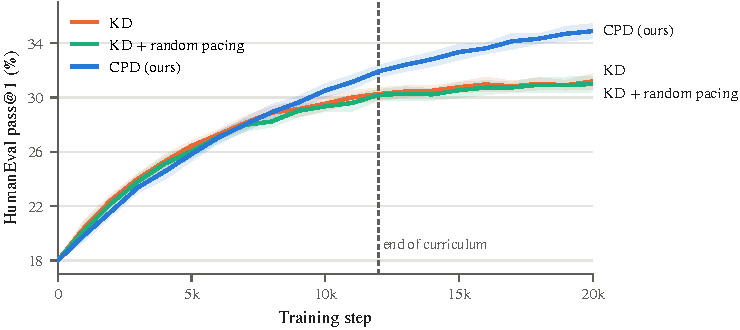
\includegraphics[width=0.85\linewidth]{figures/fig_curves.pdf}
\caption{HumanEval pass@1 of the 1.3B student during training (mean of three seeds; bands show the range over seeds). The dashed line marks the end of the curriculum at step $S = 12$k.}
\label{fig:curves}
\end{figure}

\section{Analysis}
\label{sec:analysis}

\paragraph{Where does the gain come from?}
We split the HumanEval problems into four quartiles of equal size by the difficulty score of Eq.~(\ref{eq:difficulty}), computed with the teacher exactly as for the training data.
Figure~\ref{fig:difficulty} shows the pass@1 of the 1.3B student in each quartile.
On the easiest quartile, CPD and KD are within one point of each other.
The gain grows with difficulty: on the hardest quartile, CPD solves 9.1\% of the problems against 2.4\% for KD.
This fits the motivation of Section~\ref{sec:intro}: problems that are out of reach early in training become learnable once the student has mastered the easier ones.
CPD also makes the student more robust to distribution shift, because it meets hard problems only when it is ready for them.

\begin{figure}[t]
\centering
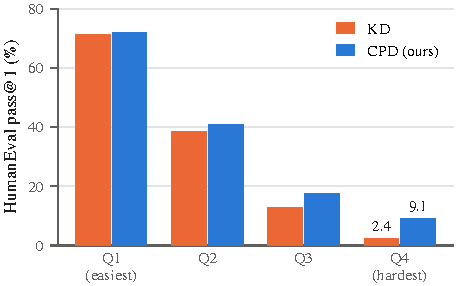
\includegraphics[width=0.62\linewidth]{figures/fig_difficulty.pdf}
\caption{HumanEval pass@1 of the 1.3B student by difficulty quartile (Q1 easiest, Q4 hardest), KD and CPD.}
\label{fig:difficulty}
\end{figure}

\paragraph{Which part of the score matters?}
The ablations in Table~\ref{tab:ablation} (Appendix~\ref{app:results}) remove one term of Eq.~(\ref{eq:difficulty}) at a time. % R1-09 Moved the ablation rows to Table 3 in Appendix B.
Without the pass-rate term, pass@1 on HumanEval drops by 1.3 points; without the likelihood term, it drops by 2.1 points.
Each term alone still beats KD, and the two together are best.

\paragraph{Sensitivity.}
CPD is not sensitive to its pacing parameters.
Linear pacing, a larger starting pool ($\lambda_0 = 0.5$) and a shorter curriculum ($S = 6$k) all lose less than 1.5 points against the default, and all of them stay above KD.
The temperature matters more: with $T = 1$ the soft targets are close to one-hot, and pass@1 drops by 1.7 points.

\paragraph{Which difficulty score?}
We also tried two other ways to order the data, keeping the pacing of Eq.~(\ref{eq:pacing}) fixed.
Ordering by the length of the reference solution gives 32.0\% pass@1 on HumanEval for the 1.3B student, and ordering by the student's own loss, recomputed every 2k steps, gives 32.6\%.
Both are better than KD (31.2\%) but well below CPD (34.9\%).

\paragraph{What do easy and hard problems look like?}
The easiest fifth of the training set, where CPD starts, consists mostly of string and list manipulation with reference solutions of fewer than ten lines.
The hardest tenth is dominated by problems that need recursion, dynamic programming or the parsing of structured input, and by problems whose descriptions leave edge cases implicit.
The two terms of Eq.~(\ref{eq:difficulty}) agree only moderately (Spearman correlation 0.41): the likelihood term ranks long solutions as hard, while the pass-rate term picks out short problems that the teacher nevertheless gets wrong.

\paragraph{How do the failures change?}
We sorted the failed HumanEval completions of the 1.3B student into three classes: code that does not parse, code that raises an exception, and code that runs but returns a wrong answer.
CPD reduces all three, but not equally.
Parse errors fall only slightly, from 4.9\% to 4.4\% of all completions, since both students learn the syntax early on.
Exceptions fall from 21.3\% to 19.8\%, and wrong answers from 42.6\% to 40.9\%.
The largest drop is in wrong answers, which suggests that the curriculum mainly helps the student get the logic of harder problems right rather than their syntax.

\section{Conclusion}
\label{sec:conclusion}

We presented CPD, a curriculum for distilling code models that orders the training problems by a difficulty score computed once with the teacher and adds harder problems at a controlled pace.
CPD costs about 9\% more than standard KD, needs no change to the loss or the model, and improves pass@1 at both student sizes we tried, mostly on the hardest problems.

Our study has limitations.
We used one teacher, one programming language and two student sizes, and we did not tune the pacing function for each size.
The pass-rate term of the score needs unit tests; for data without tests only the likelihood term is available, which loses 1.3 points on HumanEval in our ablation.
Whether the same score works for other languages, and for students distilled from several teachers, is left for future work.
We will release our code and the difficulty scores of the training set upon publication.

\section*{Reproducibility statement}

Section~\ref{sec:method} and Algorithm~\ref{alg:cpd} describe the method in full, and Appendix~\ref{app:impl} lists every hyper-parameter.
The training set is built from public sources as described in Section~\ref{sec:experiments}.
Both benchmarks are public, and every number we report is a mean over three seeds.

\bibliography{references}
\bibliographystyle{iclr2027_conference}

\appendix

\section{Implementation details}
\label{app:impl}

Table~\ref{tab:hparams} lists the hyper-parameters shared by all runs.
Sampling for the pass rate $s(x)$ uses temperature 0.8 and nucleus sampling with threshold 0.95.
Unit tests run in a sandbox with a limit of 10 seconds per problem.
Scoring the training set and distilling the students used 8 GPUs with 80\,GB of memory each.

\begin{table}[h]
\caption{Hyper-parameters shared by all runs.}
\label{tab:hparams}
\centering
\begin{tabular}{lc}
\toprule
Hyper-parameter & Value \\
\midrule
Training steps $N$ & 20k \\
Batch size & 256 \\
Peak learning rate $\eta$ & $2 \times 10^{-4}$ \\
Warm-up steps & 500 \\
Weight decay & 0.1 \\
Maximum sequence length & 2048 \\
Loss weight $\alpha$ & 0.7 \\
Teacher samples per problem $k$ & 8 \\
\bottomrule
\end{tabular}
\end{table}

\section{Additional results}
\label{app:results}

The standard deviation over three seeds is between 0.2 and 0.6 points for every entry of Table~\ref{tab:main}.
CPD beats KD in each of the three seeds, at both student sizes and on both benchmarks.

% R1-09 Moved the ablation rows to Table 3 in Appendix B.
\begin{table}[h]
\caption{Ablations of CPD for the 1.3B student. Pass@1 (\%), mean of three seeds; the default CPD reaches 34.9 on HumanEval and 43.0 on MBPP.}
\label{tab:ablation}
\centering
\begin{tabular}{llcc}
\toprule
Student & Method & HumanEval & MBPP \\
\midrule
1.3B & CPD, no pass-rate term ($\beta = 0$) & 33.6 & 42.1 \\
 & CPD, no likelihood term & 32.8 & 41.5 \\
 & CPD, linear pacing ($p = 1$) & 34.1 & 42.4 \\
 & CPD, $\lambda_0 = 0.5$ & 33.9 & 42.6 \\
 & CPD, $S = 6$k & 33.5 & 42.0 \\
 & CPD, $T = 1$ & 33.2 & 41.9 \\
 & CPD, $T = 4$ & 34.3 & 42.7 \\
\bottomrule
\end{tabular}
\end{table} % R1-09 Moved the ablation rows to Table 3 in Appendix B.

\end{document}
